\documentclass[12pt]{article}
\usepackage[utf8]{inputenc}
\usepackage{hyperref}
\usepackage{tikz}
\usetikzlibrary{arrows.meta, positioning}

\title{The Beauty of Abstraction}
\author{Shaan Fulton}
\date{\today}

\begin{document}

\maketitle

\section*{Civilization}

How have humans created so much compared to other living beings? We aren't particularly large. There are larger animals. We are dexterous, but what about the apes? They too are dexterous. But what about intelligence? The Neanderthals were intelligent. Where are their skyscrapers?

And all of this is quite new. For millions of years early humans lacked any large, complex, advanced civilizations. What changed?

We started growing plants and living close to one another. We used our intelligence to start telling stories. And these stories powered \textbf{the greatest invention in human history: Abstraction.}

\begin{center}
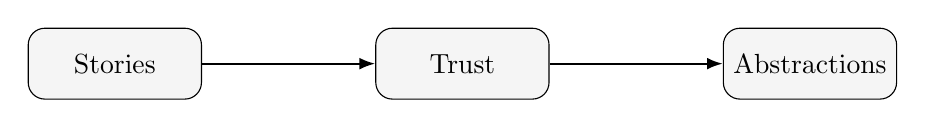
\begin{tikzpicture}[
  node distance=2.2cm,
  every node/.style={draw, rounded corners=6pt, minimum width=2.2cm, minimum height=0.9cm, font=\normalsize, fill=gray!8},
  arrow/.style={-{Latex[length=2mm]}, thick}
]

\node (stories) {Stories};
\node (trust) [right=of stories] {Trust};
\node (abs) [right=of trust] {Abstractions};

\draw[arrow] (stories) -- (trust);
\draw[arrow] (trust) -- (abs);

\end{tikzpicture}
\end{center}

I do not know how to build a skyscraper. No one does. But some humans know how to pour concrete. Some know how to design a foundation so the skyscraper will not fall. Others know how to convince all these people to build a skyscraper for them. The concrete pourer doesn't have to know how the foundation works: this is abstracted from him. The engineer doesn't have to know how the concrete is poured: this is abstracted from him.

These are layers of abstraction. The independent actors within this system of abstractions trusts one another through the stories they tell. And by abstracting away different pieces of the skyscraper, a very complex task can be broken up into a set of rather simple ones.

\begin{quote}
\textbf{Abstraction} is the process of considering something independently of its associations.
\end{quote}

By breaking up a complex system into a number of distinct abstractions, where every abstraction is one which an individual human can control without consideration of its associations, humanity can accomplish anything.

\section*{Abstractions and Computers}

Computers are complex. We employ abstractions to make them usable.

\begin{document}

\begin{center}
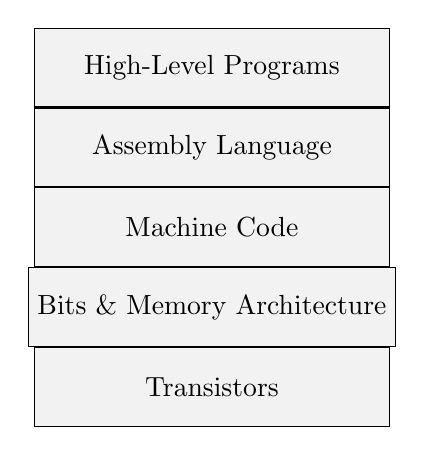
\begin{tikzpicture}[
  layerbox/.style={draw, fill=gray!10, minimum width=4.5cm, minimum height=1cm, font=\normalsize, align=center}
]

\node[layerbox] (highlevel) {High-Level Programs};
\node[layerbox, below=0cm of highlevel] (assembly) {Assembly Language};
\node[layerbox, below=0cm of assembly] (machine) {Machine Code};
\node[layerbox, below=0cm of machine] (bits) {Bits \& Memory Architecture};
\node[layerbox, below=0cm of bits] (transistors) {Transistors};

\end{tikzpicture}
\end{center}

In each layer, an individual can work without considering the possibilities of the layers above or the complexity of the layers below.

But this idea extends beyond this simple architectural diagram. Good abstraction is useful across computer science. Consider a react app, for instance. The frontend developer does not need to know how the button component renders beautifully on any sized web display, or how the server handles their \texttt{submit-contact} request. They just need to know what it does in the context of their needs: they need a user input and to collect data.

Good abstraction goes beyond making complex projects possible. The scope of the project can easily be extended to the end-user. \textbf{Good design is good abstraction}. The end-user should only have to care about what they provide. In a bank application, this is a desired withdrawal amount. That's it. The most perfect interface is the one that abstracts everything else away.

But it goes beyond this. Ultimately, it's just a matter of what value the individual in our system of abstractions is optimized to provide. The user might not even be the one to decide if a withdrawal should be made or not. In fact, in a perfect system of abstractions perhaps the user is only concerned with their work and leisure. They do not worry about making withdrawals. At some point in the layers there is a budgeting system. At another point, a shopping assistant. Etcetera.

There is some beauty in this form of efficiency. Perhaps it is also somewhat distopian. I think people value knowing what is at the "back of things." Life itself is in some sense a great abstraction. Much of philosophy is some attempt to uncover this. The Kantian noumenon comes to mind, as well as Plato's Allegory of the Cave. Perhaps it was all designed this way in the name of efficiency. I suppose also that the desire to know what is at the "back of things" which motivates a study in philosophy may also motivate a study in computer science.

\end{document}

